% Options for packages loaded elsewhere
\PassOptionsToPackage{unicode}{hyperref}
\PassOptionsToPackage{hyphens}{url}
%
\documentclass[
  9pt,
]{article}
\usepackage{amsmath,amssymb}
\usepackage{iftex}
\ifPDFTeX
  \usepackage[T1]{fontenc}
  \usepackage[utf8]{inputenc}
  \usepackage{textcomp} % provide euro and other symbols
\else % if luatex or xetex
  \usepackage{unicode-math} % this also loads fontspec
  \defaultfontfeatures{Scale=MatchLowercase}
  \defaultfontfeatures[\rmfamily]{Ligatures=TeX,Scale=1}
\fi
\usepackage{lmodern}
\ifPDFTeX\else
  % xetex/luatex font selection
\fi
% Use upquote if available, for straight quotes in verbatim environments
\IfFileExists{upquote.sty}{\usepackage{upquote}}{}
\IfFileExists{microtype.sty}{% use microtype if available
  \usepackage[]{microtype}
  \UseMicrotypeSet[protrusion]{basicmath} % disable protrusion for tt fonts
}{}
\makeatletter
\@ifundefined{KOMAClassName}{% if non-KOMA class
  \IfFileExists{parskip.sty}{%
    \usepackage{parskip}
  }{% else
    \setlength{\parindent}{0pt}
    \setlength{\parskip}{6pt plus 2pt minus 1pt}}
}{% if KOMA class
  \KOMAoptions{parskip=half}}
\makeatother
\usepackage{xcolor}
\usepackage[left=1.3cm,right=1.3cm,top=1.5cm,bottom=0.5cm]{geometry}
\usepackage{graphicx}
\makeatletter
\def\maxwidth{\ifdim\Gin@nat@width>\linewidth\linewidth\else\Gin@nat@width\fi}
\def\maxheight{\ifdim\Gin@nat@height>\textheight\textheight\else\Gin@nat@height\fi}
\makeatother
% Scale images if necessary, so that they will not overflow the page
% margins by default, and it is still possible to overwrite the defaults
% using explicit options in \includegraphics[width, height, ...]{}
\setkeys{Gin}{width=\maxwidth,height=\maxheight,keepaspectratio}
% Set default figure placement to htbp
\makeatletter
\def\fps@figure{htbp}
\makeatother
\setlength{\emergencystretch}{3em} % prevent overfull lines
\providecommand{\tightlist}{%
  \setlength{\itemsep}{0pt}\setlength{\parskip}{0pt}}
\setcounter{secnumdepth}{-\maxdimen} % remove section numbering
\usepackage{fancyhdr} \usepackage{graphicx} \usepackage{eurosym} \usepackage{datetime} \usepackage{booktabs,xcolor} \pagestyle{fancy} \fancypagestyle{plain}{\pagestyle{fancy}} \pagenumbering{gobble} \renewcommand\thefootnote{\textcolor{black}{\arabic{footnote}}} \usepackage{pagecolor} \pagecolor{white} \usepackage{fourier} \usepackage[fontsize=8.7pt]{scrextend} \usepackage{float} \restylefloat{table} \usepackage{xcolor} \usepackage{multicol} \newcommand{\hideFromPandoc}[1]{#1} \hideFromPandoc{ \let\Begin\begin \let\End\end } \usepackage{caption} \captionsetup{skip=0pt} \usepackage{hyperref} \usepackage{array} \usepackage{varwidth} \hypersetup{ colorlinks=true, linkcolor=blue, filecolor=magenta, urlcolor=cyan, } \urlstyle{same} \usepackage{enumitem} \setlist{leftmargin=*} \pagenumbering{gobble} \usepackage{numprint} \usepackage{fbox}
\ifLuaTeX
  \usepackage{selnolig}  % disable illegal ligatures
\fi
\IfFileExists{bookmark.sty}{\usepackage{bookmark}}{\usepackage{hyperref}}
\IfFileExists{xurl.sty}{\usepackage{xurl}}{} % add URL line breaks if available
\urlstyle{same}
\hypersetup{
  pdftitle={Paraguay},
  hidelinks,
  pdfcreator={LaTeX via pandoc}}

\title{Paraguay}
\author{}
\date{\vspace{-2.5em}}

\begin{document}
\maketitle

\definecolor{bondiblue}{rgb}{0.0, 0.58, 0.71}
\definecolor{steelblue}{rgb}{0.27, 0.51, 0.71}
\definecolor{brickred}{rgb}{0.8, 0.25, 0.33}
\newcommand\boldblue[1]{\textcolor{bondiblue}{\textbf{#1}}}

This two-page brief provides the 2020 Human Capital Index (HCI) released
in September 2020, and a set of complementary indicators. The HCI
measures the amount of human capital that a child born today can expect
to attain by age 18. It conveys the productivity of the next generation
of workers compared to a benchmark of complete education and full
health. Although the effects of COVID-19 on this index are yet to be
measured due to the lack of data, we expect the post-pandemic HCI to be
relatively lower due to the deep learning and health losses globally.
\textbf{Data collection efforts to allow updates to the HCI remain
critical for all countries to inform policies and programs to address
the setbacks to human capital.}

\begin {multicols}{2}

\hypertarget{section}{%
\subsubsection{\texorpdfstring{\textcolor{bondiblue}{\textbf{T\small{HE HUMAN CAPITAL INDEX}}}}{}}\label{section}}

A child born in Paraguay just before the pandemic will be \textbf{53
percent} as productive when she grows up as she could be if she enjoyed
complete education and full health.

This is lower than the average for the Latin America \& Caribbean region
(56 percent) and Upper Middle Income countries (56 percent).

\hypertarget{section-1}{%
\subsubsection{\texorpdfstring{\textcolor{bondiblue}{\textbf{T\small{HE HUMAN CAPITAL INDEX COMPONENTS}}}}{}}\label{section-1}}

\begin{itemize}
\item
  \textbf{Probability of Survival to Age 5.} Of every 100 children born
  in Paraguay, \textbf{98} survive to age 5.
\item
  \textbf{Expected Years of School.} In Paraguay, a child who starts
  school at age 4 can expect to complete \textbf{11.3 years} of school
  by her 18th birthday.
\item
  \textbf{Harmonized Test Scores.} Students in Paraguay score
  \textbf{386} on a scale where 625 represents advanced attainment and
  300 represents minimum attainment.
\item
  \textbf{Learning-adjusted Years of School.} Factoring in what children
  actually learn, expected years of school is only \textbf{7 years}.
\item
  \textbf{Adult Survival Rate.} Across Paraguay, \textbf{86 percent} of
  15-year olds will survive until age 60. This statistic is a proxy for
  the range of health risks that a child born today would experience as
  an adult under current conditions.
\item
  \textbf{Fraction of Children Under 5 Not Stunted.} Approximately
  \textbf{94} out of 100 children are \textbf{not} stunted.This means
  that \textbf{6} out of 100 children are at risk of cognitive and
  physical limitations that can last a lifetime.
\end{itemize}

\hypertarget{section-2}{%
\subsubsection{\texorpdfstring{\textcolor{bondiblue}{\textbf{T\small{HE HUMAN CAPITAL UTILIZATION}}}}{}}\label{section-2}}

The returns on human capital are realized when individuals predominantly
utilize that capital through work. Consequently, we introduce a
utilization-adjusted Human Capital Index (UHCI) that accounts for
underutilization of human capital in the labor market by taking into
account the proportion of the employed working-age population.

\begin{itemize}
\item
  In Paraguay, adjusting the HCI for utilization leads to a decrease to
  37 percent. This suggests that nearly less than half of Paraguay's
  population is unable to fully leverage their skills and knowledge to
  contribute effectively to the economy.
\item
  Comparing by gender, the adjusted utilization of human capital is
  higher for males (43 percent) than for females (31 percent)
\end{itemize}

\vspace{-0.5mm}
\begin{table}[H]
\renewcommand{\tabcolsep}{0.8mm}
\begin{tabular}{m{0.3\textwidth}>{\centering\arraybackslash}m{0.054\textwidth}>{\centering\arraybackslash}m{0.054\textwidth}>{\centering\arraybackslash}m{0.054\textwidth}}
\\\textbf{     }   &    &             &  \\ \hline
                         &      &              & \\
\textbf{ Human Capital and Utilization   } & \textbf{ Boys} & \textbf{ Girls} &  \textbf{ Overall} \\\hline
\vspace{-1mm} \\
Human Capital Index (HCI) &   0.53 &   0.53 &    0.53\\
Utilization of Human Capital Index (UHCI) & 0.43  &  0.31 & 0.37 \\
                         & \multicolumn{1}{l}{} & \multicolumn{1}{l}{} &    
\vspace{-4mm}
\\\hline
\end{tabular}
\vspace{1mm} 
\end{table}

\begin{flushright}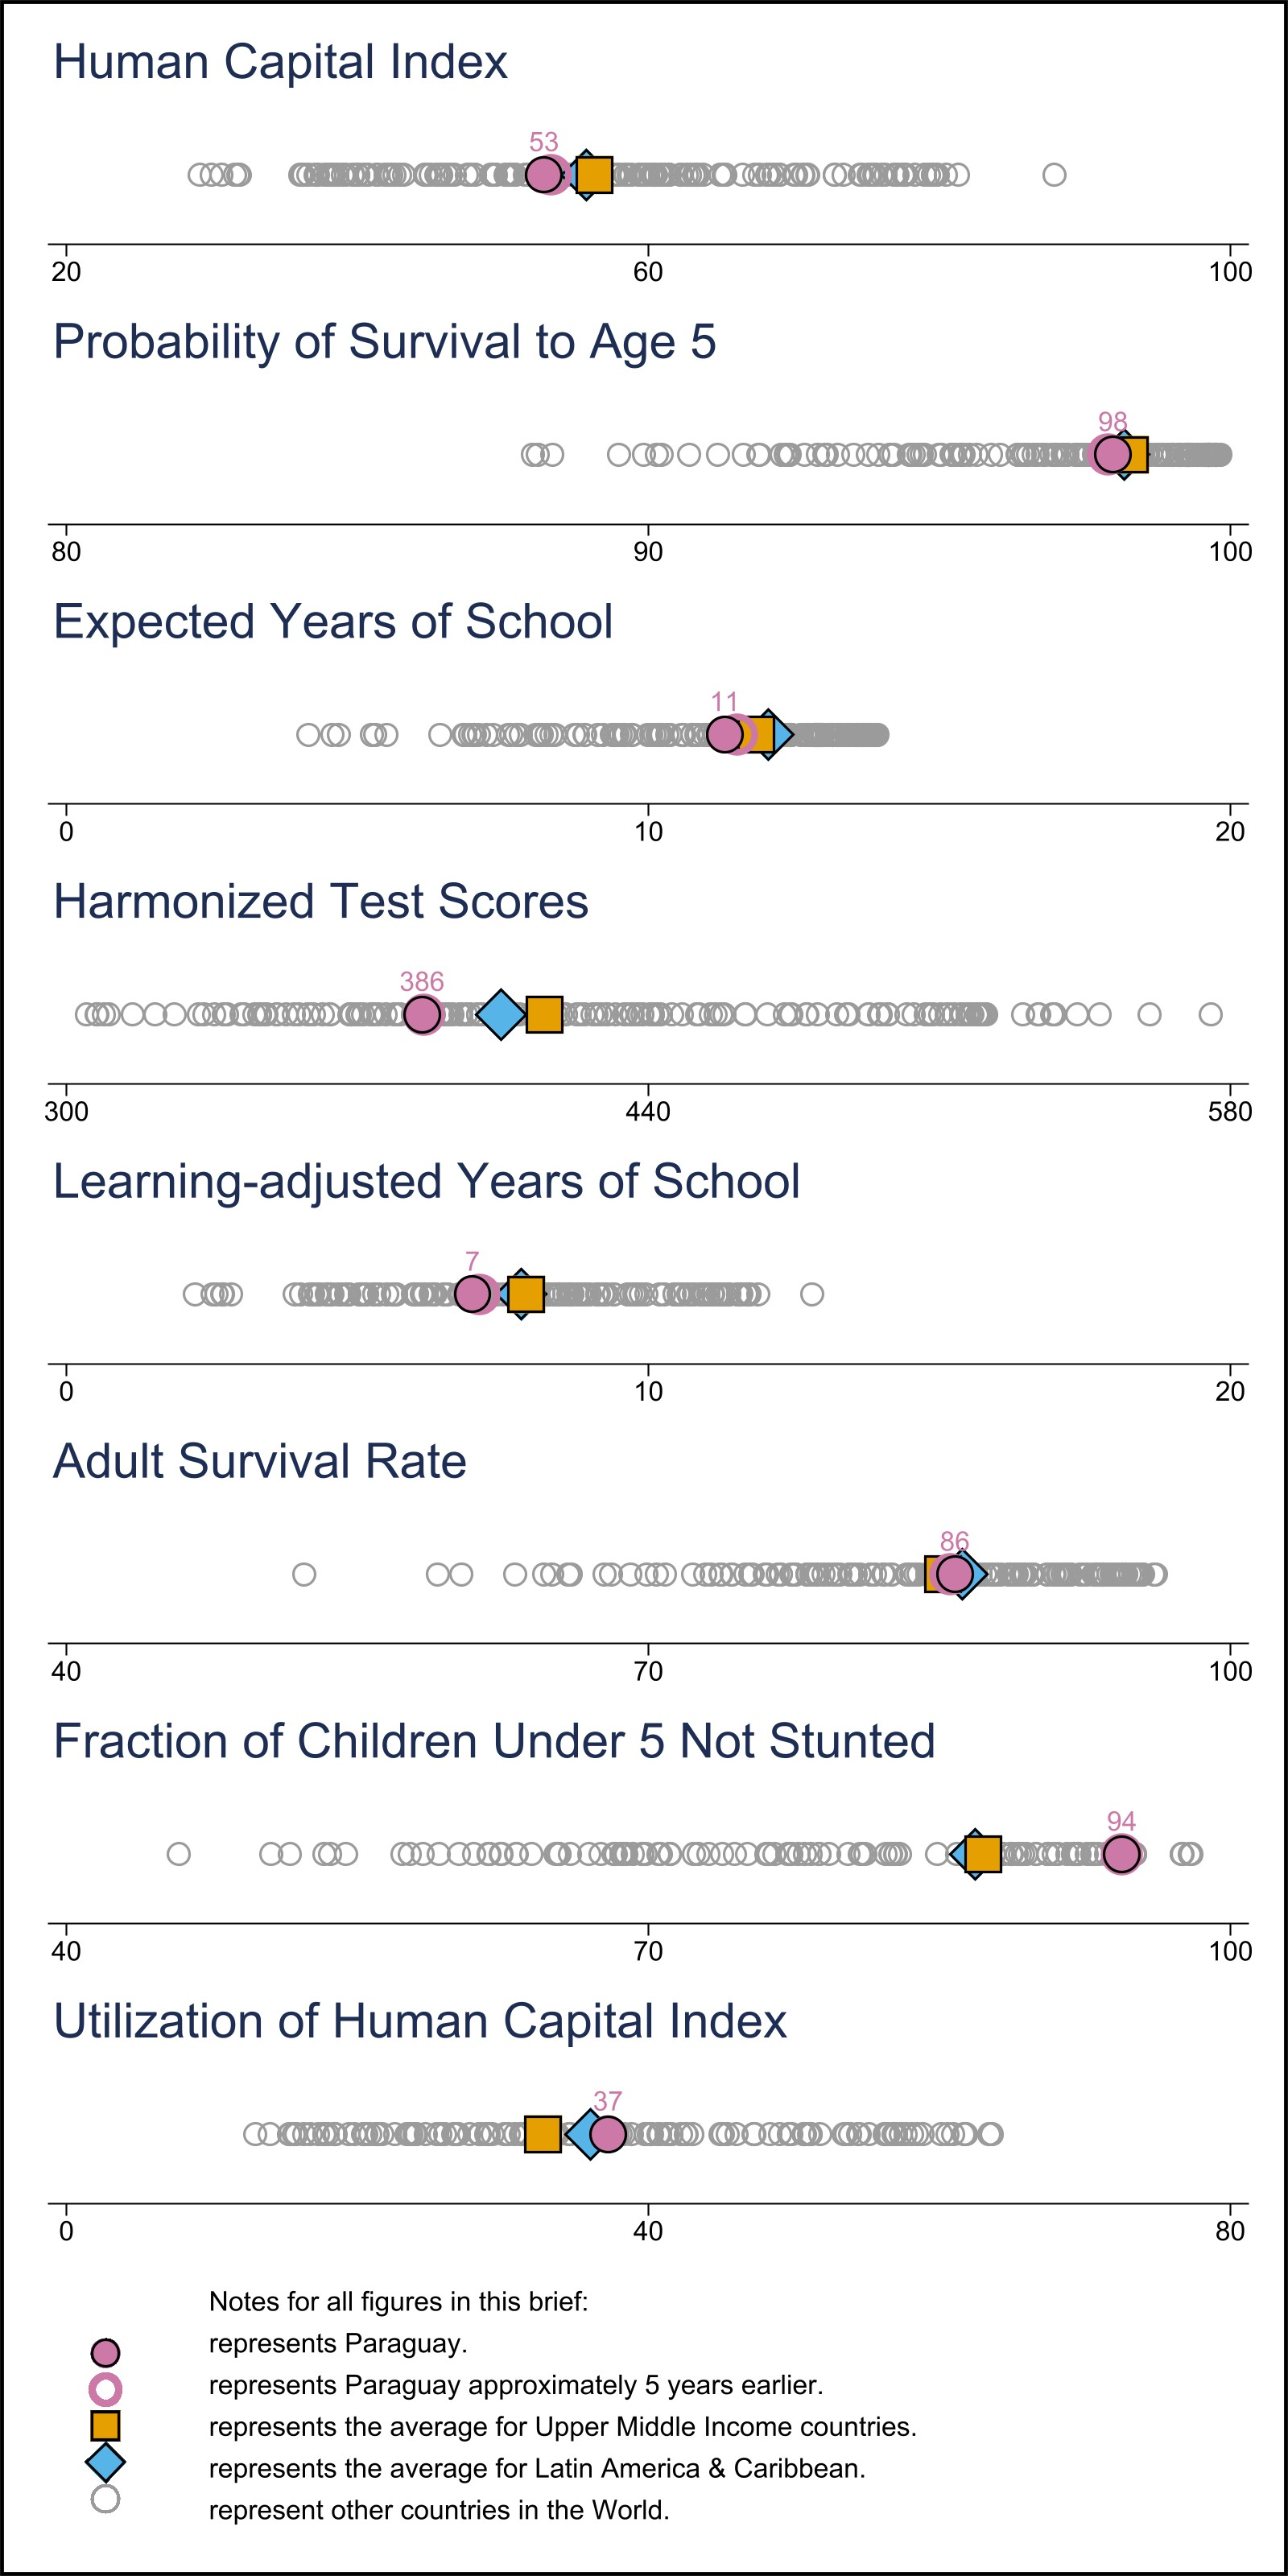
\includegraphics[height=0.9\textheight]{Graphs/p1_PRY_all} \end{flushright}

\vfill

\end {multicols}

\newpage

\vspace{3mm}

Human capital, a crucial ingredient for economic growth, is
multi-dimensional and cumulatively built over the lifecycle. Due to the
slow-moving nature of the HCI, an additional set of Human Capital
Complementary Indicators (HCCIs) offer a snapshot of proximate
dimensions of human capital in Paraguay that can be monitored to measure
simultaneous progress in intermediate outcomes. These selected HCCIs are
based on the latest available data (\emph{italicized} and shown in
parentheses) and benchmarked against regional and country income group
averages. \textbf{They highlight where there is need for investment in
people in each stage of life and for data collection and updates for
evidence-based policy making.}

\vspace{1mm}

\begin {multicols}{2}

\hypertarget{section-3}{%
\subsubsection{\texorpdfstring{\textcolor{bondiblue}{\textbf{E\small{ARLY CHILDHOOD}}}}{}}\label{section-3}}

\begin{itemize}
\item
  \textbf{Neonatal mortality rate (deaths per 1,000 live births).} The
  neonatal mortality rate is \textbf{10 per 1,000 live births}
  (\emph{2021}). The indicator is similar to both the regional average
  (10) and the income group average (10).
\item
  \textbf{Participation rate in organized learning (\% of children one
  year before the official primary entry age).} As in (\emph{2020}) ,
  \textbf{77 percent} of children one year before the official primary
  entry age participate in an organized learning program.. The indicator
  is both below the regional average (88\%) and the income group average
  (84\%).
\item
  \textbf{Diphtheria vaccination (\%).} Diphtheria vaccine coverage is
  \textbf{70 percent} (\emph{2021}). The indicator is lower than both
  the regional average (81\%) and the income group average (87\%).
\end{itemize}

\hypertarget{section-4}{%
\subsubsection{\texorpdfstring{\textcolor{bondiblue}{\textbf{S\small{CHOOL AGE}}}}{}}\label{section-4}}

\begin{itemize}
\item
  \textbf{Child mortality (deaths per 1,000 youth aged 5).} ~The
  mortality rate at ages 5--14 is \textbf{3 per 1,000 children aged 15}
  (\emph{2021}). The indicator is similar to both the regional average
  (3) and the income group average (3).
\item
  \textbf{Schools with basic hygiene services (\%).} The share of
  schools with handwashing facilities with water and soap available is
  \textbf{62 percent} (\emph{2020}). The indicator is both below the
  regional average (76\%) and the income group average (80\%).
\item
  \textbf{Repetition in primary education (\%).} As in \emph{2020},
  \textbf{0 percent} of students in primary education remained in the
  same grade in the following school year. The indicator is lower than
  both the regional average (2\%) and the income group average (2\%).
\end{itemize}

\hypertarget{section-5}{%
\subsubsection{\texorpdfstring{\textcolor{bondiblue}{\textbf{Y\small{OUTH}}}}{}}\label{section-5}}

\begin{itemize}
\item
  \textbf{Youth literacy rate (\%).} The literacy rate for youth ages
  15-24 years is \textbf{99 percent} (\emph{2021}). The indicator is
  higher than both the regional average (98\%) and the income group
  average (98\%).
\item
  \textbf{Youth mortality (deaths per 1,000 youth aged 15).} ~The
  mortality rate at ages 15--24 is \textbf{11 per 1,000 youth aged 15}
  (\emph{2021}). The indicator is both above the regional average (10)
  and the income group average (9).
\item
  \textbf{Youth unemployment (\%).} The unemployment rate among youth
  ages 15-24 is \textbf{16 percent} (\emph{2023}). The indicator is
  lower than both the regional average (21\%) and the income group
  average (23\%).
\end{itemize}

\hypertarget{section-6}{%
\subsubsection{\texorpdfstring{\textcolor{bondiblue}{\textbf{A\small{DULTS \& ELDERLY}}}}{}}\label{section-6}}

\begin{itemize}
\item
  \textbf{Labor force participation (\%).} The labor force participation
  as percentage of the working population is \textbf{75 percent}
  (\emph{2022}). The indicator is higher than both the regional average
  (68\%) and the income group average (65\%).
\item
  \textbf{Adult unemployment (\%).} The unemployment rate among adults
  more than 25 years old is \textbf{5 percent} (\emph{2023}). The
  indicator is both below the regional average (7\%) and the income
  group average (9\%).
\item
  \textbf{Health care facilities with basic sanitation services (\%).}
  The share of health care facilities with improved sanitation
  facilities is \textbf{26 percent} (\emph{2021}). The indicator is
  higher than the regional average (20\%) but lower than the income
  group average (37\%).
\end{itemize}

\begin{flushright}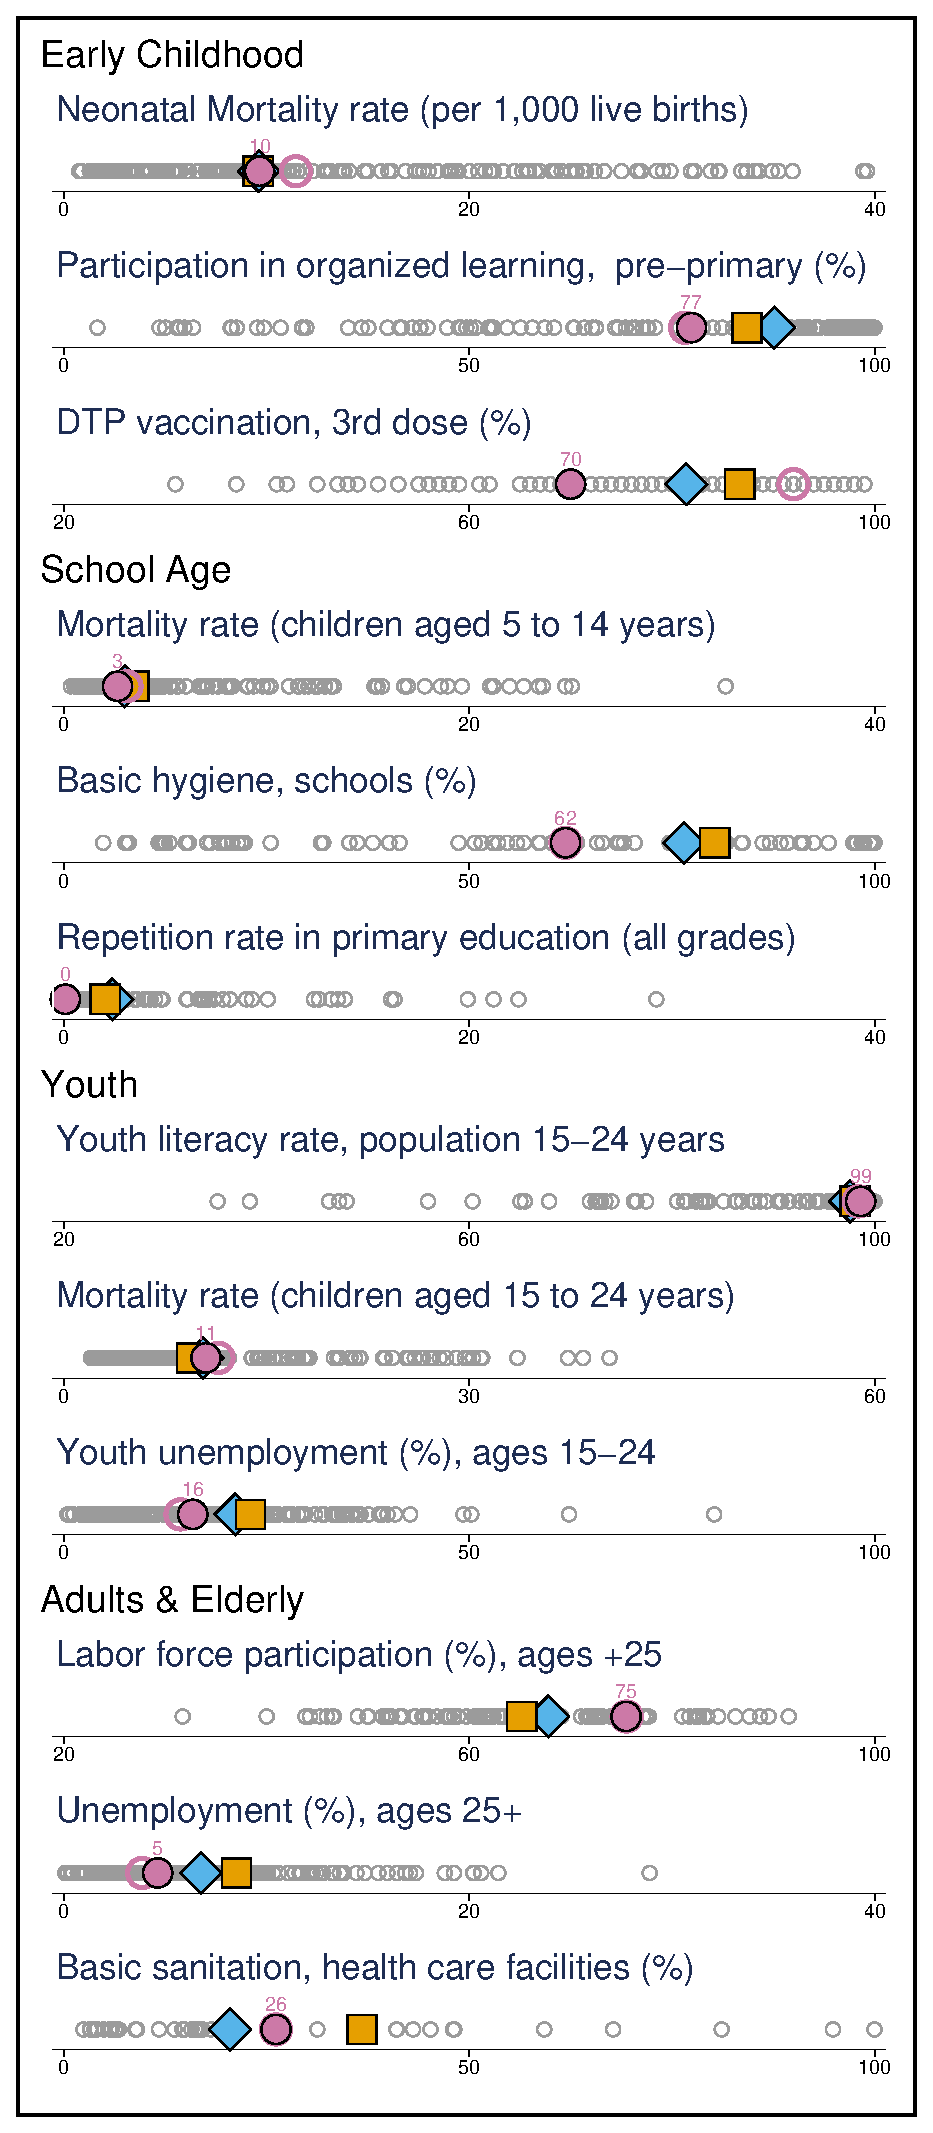
\includegraphics[height=0.88\textheight]{Graphs/p2_PRY_stages} \end{flushright}

\end {multicols}

\end{document}
